\documentclass[11pt,a4paper]{article}
\usepackage[utf8]{inputenc}
\usepackage[margin=2.5cm]{geometry}
\usepackage{graphicx}
\usepackage{hyperref}
\usepackage{booktabs}
\usepackage{amsmath}
\usepackage{amssymb}
\usepackage{float}
\usepackage{enumitem}
\usepackage{xcolor}

\title{Natural Language Processing Coursework}
\author{Jack Xiuqi Zhang\\CID: 02372321}
\date{\today}

\begin{document}

\maketitle
\tableofcontents
\newpage

%==============================================================================
\section{Exercise 1: Critical Paper Review}
%==============================================================================

\subsection{Q1: Primary Contributions}

The paper addresses an under-explored problem in NLP: detecting Patronising and Condescending Language (PCL) towards vulnerable communities in media discourse.
The authors introduced the \textit{Don't Patronize Me!} dataset, containing 10637 paragraphs concerning vulnerable social groups, annotated for both PCL presence and specific PCL categories.
The authors evaluate several baseline models, including SVM-based methods, BiLSTM, and BERT variants, with RoBERTa-base achieving the best performance (F1 = 70.63\%) on binary PCL classification.
The authors also proposed a taxonomy of PCL categories, aimed to help better understand the different forms of PCL and to guide future research.

\subsection{Q2: Technical Strengths}

\begin{itemize}[noitemsep]
    \item The dataset draws from news sources across 20 English-speaking countries and covers 10 distinct vulnerability keywords, ensuring diversity and representativeness.
    \item The two step annotation scheme, which first identifies PCL presence and then categorises PCL spans, enables both binary classification and fine-grained category analysis.
    \item The annotation process used a rigorous two-step methodology, where the first step involved identifying the presence of PCL and the second step involved categorising the type of PCL, which allows for more detailed analysis.
    \item The paper establishes clear benchmarks through comprehensive evaluation of both traditional methods (SVM, BiLSTM) and transformer-based models (BERT, RoBERTa, DistilBERT).
\end{itemize}

\subsection{Q3: Key Weaknesses}

\begin{itemize}[noitemsep]
    \item The dataset is relatively small for training large transformer-based models, particularly for underrepresented categories (e.g., \textit{"The poorer, the merrier"} contains only 64 samples), risking overfitting and limiting generalisation.
    \item The experiments use only paragraph-level classification, the available span-level annotations are not utilised for training, potentially limiting the models' ability to learn fine-grained PCL patterns.
\end{itemize}

\newpage
%==============================================================================
\section{Exercise 2: Exploratory Data Analysis}
%==============================================================================

\subsection{EDA Technique 1: Basic Statistical Profiling}

\subsubsection{Visual/Tabular Evidence}

\begin{figure}[H]
    \centering
    
\includegraphics[width=\textwidth]{figures/basic_statistical_profiling.png}
    \caption{Basic statistical profiling of the PCL training set. \textit{Top-left}: frequency and percentage of each of the 7 PCL label categories. \textit{Top-right}: distribution of how many labels each sample carries (multi-label distribution). \textit{Bottom}: histogram of token counts per sample with median (38) and mean (44.2) markers.}
    \label{fig:eda1}
\end{figure}

\begin{table}[H]
    \centering
    \begin{tabular}{lrr}
        \toprule
        \textbf{Metric}    & \textbf{PCL}                  & \textbf{Non-PCL} \\
        \midrule
        Sample count       & 794                           & 7{,}581          \\
        Proportion         & 9.48\%                        & 90.52\%          \\
        Imbalance ratio    & \multicolumn{2}{c}{1\,:\,9.5}                    \\
        \midrule
        Mean token count   & \multicolumn{2}{c}{44.18}                        \\
        Median token count & \multicolumn{2}{c}{38}                           \\
        Max token count    & \multicolumn{2}{c}{820}                          \\
        Std deviation      & \multicolumn{2}{c}{26.85}                        \\
        \midrule
        Vocabulary size    & \multicolumn{2}{c}{26{,}897}                     \\
        \bottomrule
    \end{tabular}
    \caption{Summary statistics for the PCL training set (8{,}375 samples total).}
    \label{tab:eda1}
\end{table}

\subsubsection{Analysis}

The basic statistical profiling reveals concrete structural challenges in the PCL dataset:

\begin{enumerate}[noitemsep]
    \item \textbf{Severe Class Imbalance.} Exactly 7{,}581 of the 8{,}375 training samples (90.5\%) are Non-PCL, leaving only 794 samples (9.5\%) as positive PCL examples — a $\sim$9.5:1 imbalance. A trivial classifier predicting ``Non-PCL'' for every input would achieve 90.5\% accuracy while having zero utility.

    \item \textbf{Within-PCL Label Sparsity.} Among the 7 PCL categories (Labels 0--6), Label\_0 is the most frequent (574 samples, 6.85\%) and Label\_5 the second most (363, 4.33\%), while Label\_6 is extremely rare with only 29 instances (0.35\%). For the binary task all labelled samples are treated uniformly as PCL\,=\,1, but this internal skew is relevant if fine-grained multi-label classification is attempted later.

    \item \textbf{Label Co-occurrence.} Of the 794 PCL samples, 551 (69.4\%) carry more than one label, with individual samples carrying up to 5 labels simultaneously. When a text is patronising, it typically exhibits multiple PCL patterns at once, indicating PCL is a multi-faceted linguistic phenomenon rather than a single discrete signal.

    \item \textbf{Right-Skewed Token Distribution.} The distribution has a median of 38 tokens, a mean of 44.18 (std 26.85), and a maximum of 820 tokens. Most samples are short-to-medium paragraphs, but a long tail of substantially longer passages must be accommodated.
\end{enumerate}

\subsubsection{Impact Statement}

\begin{itemize}[noitemsep]
    \item \textbf{Metric Selection.} With 90.5\% Non-PCL, accuracy is actively misleading. Optimisation must target \textbf{Macro-F1} with explicit tracking of the positive-class (PCL) F1. A threshold sweep on the dev set is also necessary, as the default 0.5 decision boundary is biased toward the majority class.

    \item \textbf{Loss Function.} Standard Binary Cross-Entropy will be overwhelmingly biased toward predicting ``Non-PCL''. \textbf{Weighted Binary Cross-Entropy} with \texttt{pos\_weight}\,$\approx$\,9.5 (reflecting the 9.5:1 ratio) or \textbf{Focal Loss} must be used to redirect gradient updates toward the rare PCL cases.

    \item \textbf{Sampling Strategy.} With a 1:9.5 ratio, a random mini-batch of 32 samples contains on average only $\sim$3 PCL examples — an extremely noisy training signal. \textbf{Stratified sampling} per batch is required to guarantee consistent PCL representation across training steps.

    \item \textbf{Sequence Length.} The median of 38 tokens sits well within 128 subword tokens for most transformer tokenisers, making \texttt{max\_length=128} sufficient for the bulk of the data. However, because the maximum reaches 820 tokens, \texttt{max\_length=256} is the safer default to avoid truncating the longer, elaborately structured PCL paragraphs.

    \item \textbf{Embedding Strategy.} The 26{,}897 unique tokens justify using a \textbf{pre-trained embedding} (e.g.\ GloVe or a BERT sub-word tokeniser) rather than training word embeddings from scratch on this small corpus.
\end{itemize}

\subsection{EDA Technique 2: Lexical Analysis}

\subsubsection{Visual/Tabular Evidence}

\begin{figure}[H]
    \centering
    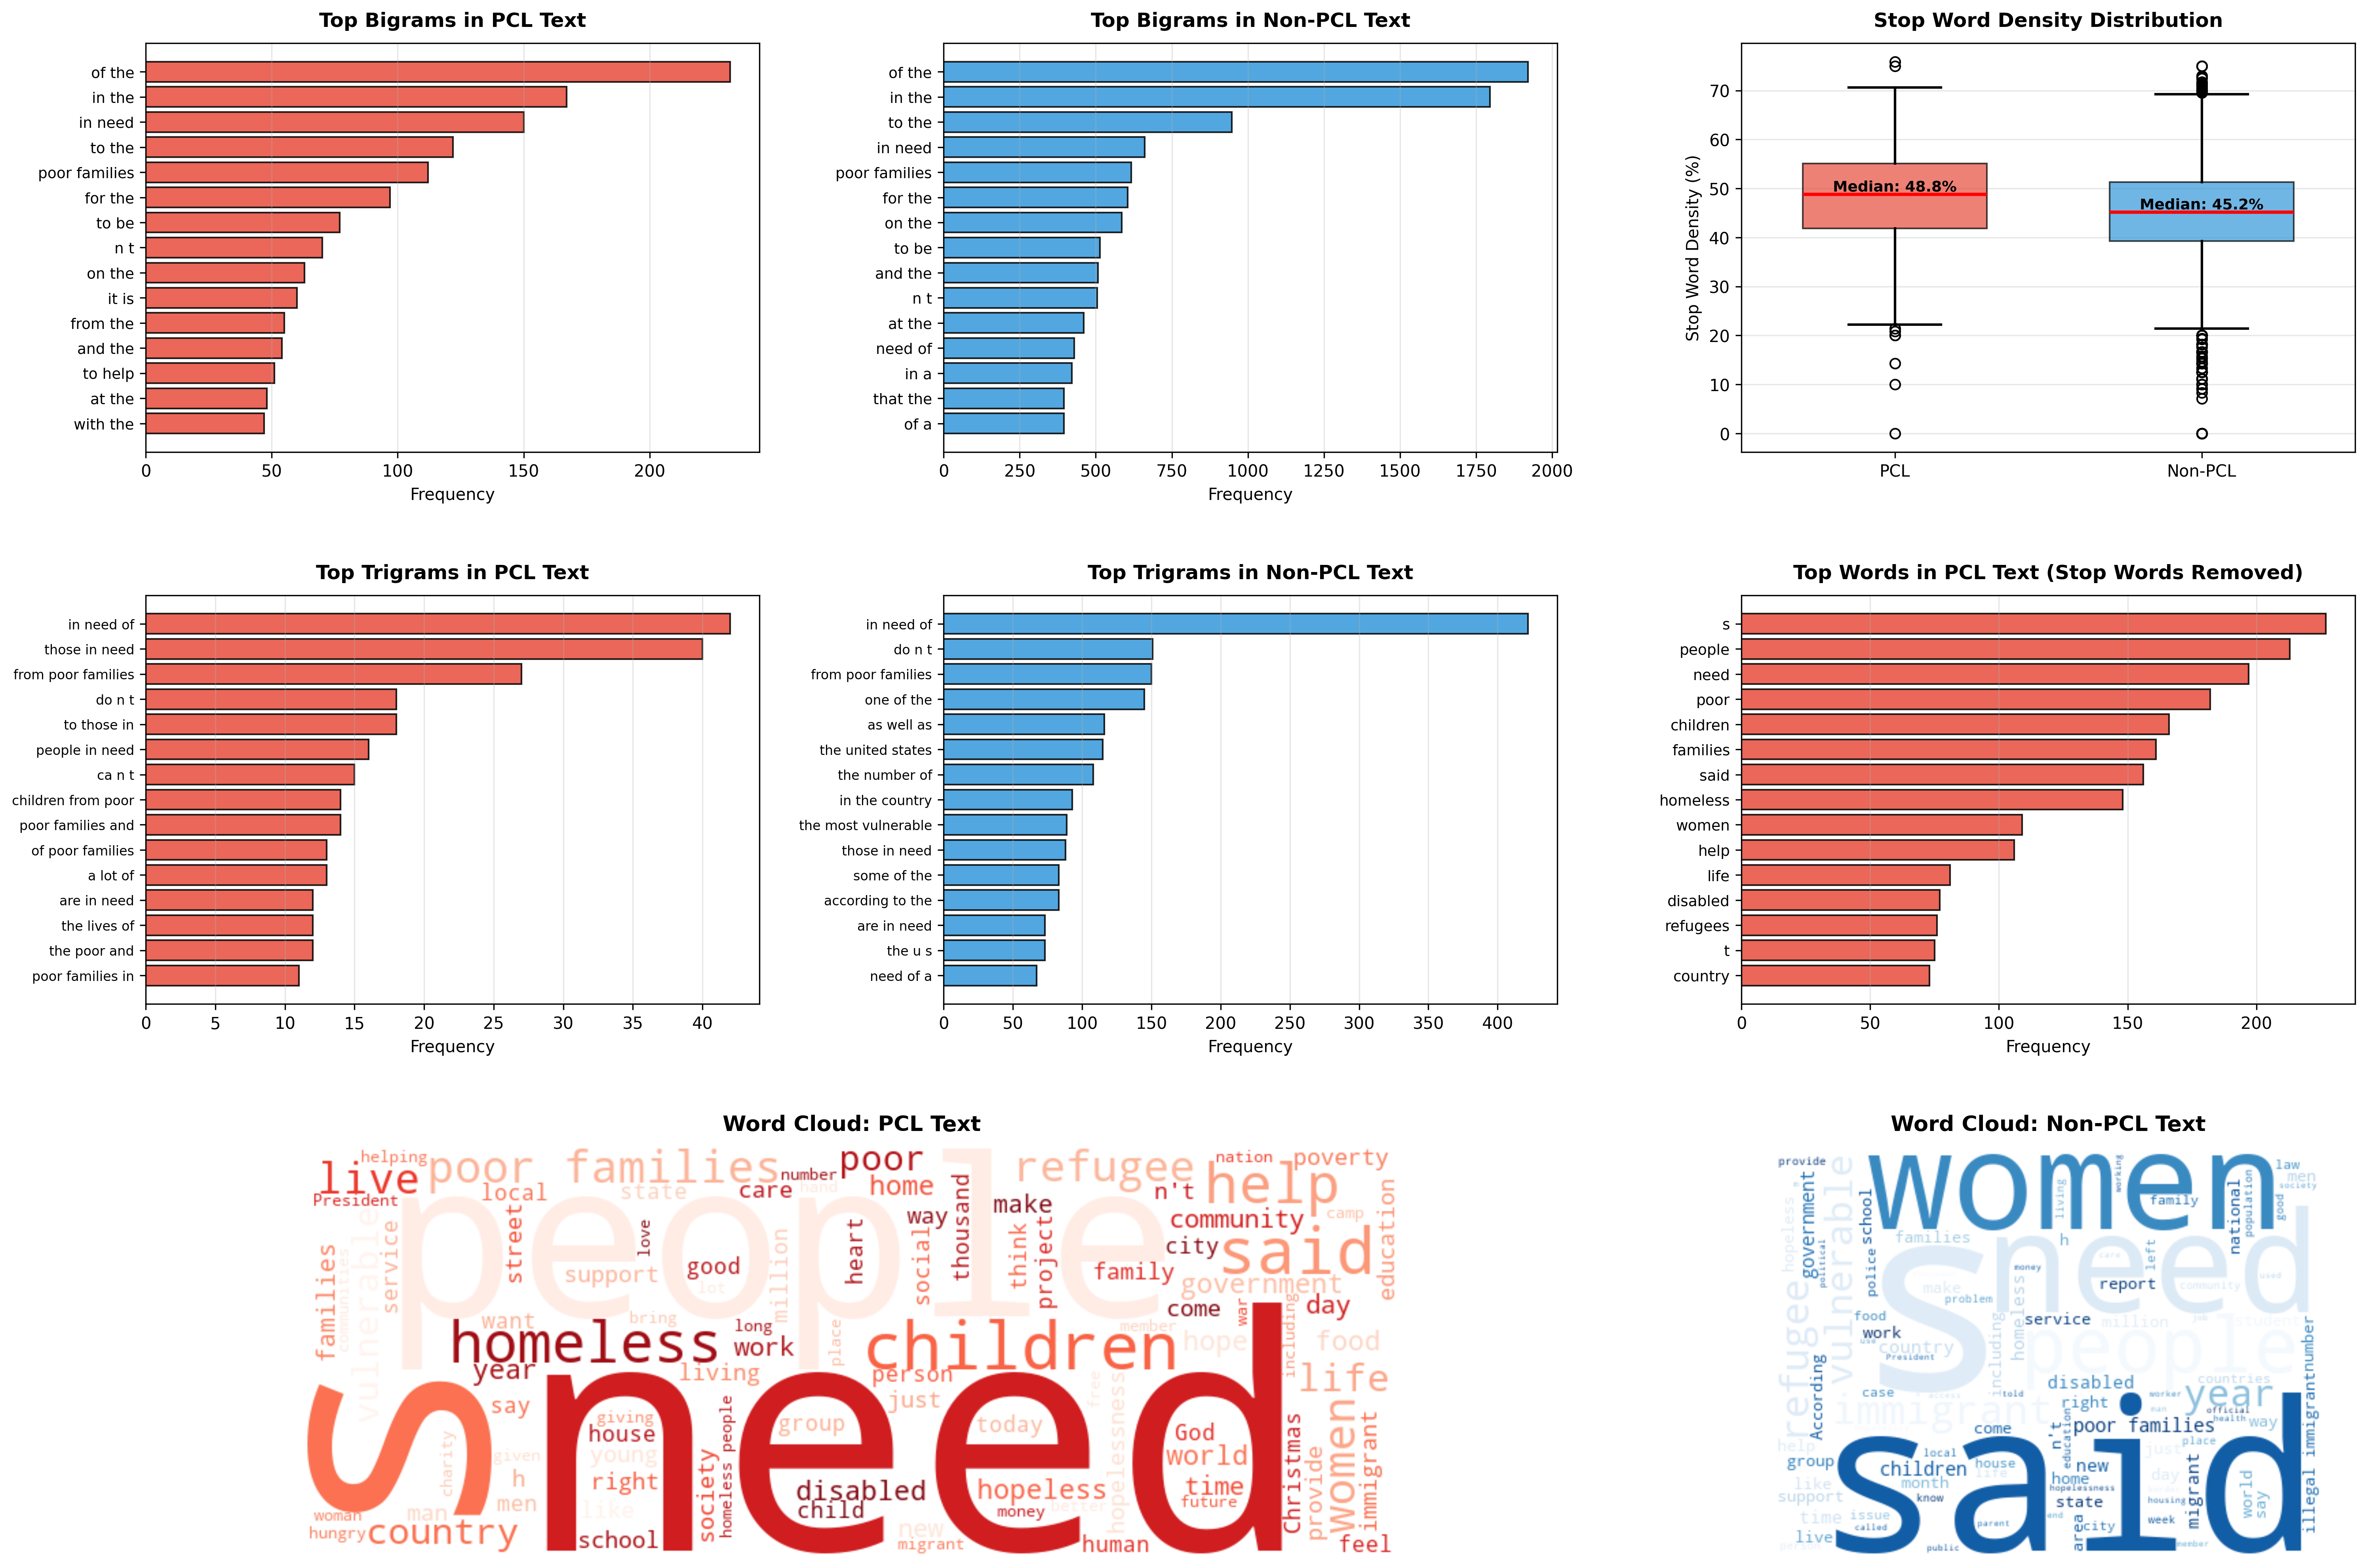
\includegraphics[width=\textwidth]{figures/lexical_analysis.png}
    \caption{Lexical analysis comparing PCL and Non-PCL text. \textit{Row 1}: top-15 bigrams per class (bar charts) and stop-word density box plots. \textit{Row 2}: top-15 trigrams per class and top-15 most frequent content words in PCL text (stop words removed). \textit{Row 3}: word clouds for PCL (red) and Non-PCL (blue) text.}
    \label{fig:eda2}
\end{figure}

\begin{table}[H]
    \centering
    \begin{tabular}{llrllr}
        \toprule
        \multicolumn{3}{c}{\textbf{PCL Trigrams}} & \multicolumn{3}{c}{\textbf{Non-PCL Trigrams}}                                                                        \\
        \cmidrule(r){1-3}\cmidrule(l){4-6}
        \textbf{Rank}                             & \textbf{Trigram}                              & \textbf{Freq.} & \textbf{Rank} & \textbf{Trigram}   & \textbf{Freq.} \\
        \midrule
        1                                         & in need of                                    & 42             & 1             & in need of         & 422            \\
        2                                         & those in need                                 & 40             & 2             & do n't             & 151            \\
        3                                         & from poor families                            & 27             & 3             & from poor families & 150            \\
        4                                         & to those in                                   & 18             & 4             & one of the         & 145            \\
        5                                         & people in need                                & 16             & 5             & the united states  & 115            \\
        \bottomrule
    \end{tabular}
    \caption{Top-5 trigrams in PCL vs Non-PCL text (raw counts). Per-sample rate for ``those in need'': PCL 0.050 vs Non-PCL 0.012 (4.2$\times$ enrichment).}
    \label{tab:trigrams}
\end{table}

\subsubsection{Analysis}

\begin{enumerate}[noitemsep]
    \item \textbf{N-gram Patterns — Vulnerability-Framing Phrases.} Top bigrams in both classes are dominated by generic English function-word pairs (``of the'', ``in the''), which carry no discriminative power on their own. The signal emerges at the trigram level. Normalising by class size, PCL text shows a \textbf{4.2$\times$ enrichment} for ``those in need'' (0.050 per PCL sample vs 0.012 for Non-PCL), and ``people in need'' appears in PCL's top 10 but not in Non-PCL's. These phrases construct a narrative of passivity and dependency — a hallmark of patronising language. Non-PCL trigrams, by contrast, are factual and geopolitical: ``the united states'', ``the number of'', ``as well as''.

    \item \textbf{Stop Word Density — PCL Uses More Elaborate Syntax.} PCL texts have a mean stop-word density of \textbf{48.47\%} (median 48.8\%) versus \textbf{45.01\%} (median 45.2\%) for Non-PCL — a gap of \textbf{3.46 percentage points} (std $\approx$9.7\% in both classes, confirming the difference is systematic). The higher density reflects the clause-heavy sentence structures of patronising language (e.g.\ \textit{``they are the ones who are in need of our help''}) compared to the more direct, noun-heavy style of factual reporting.

    \item \textbf{Distinctive Vocabulary (Per-Sample Rates).} After normalising for class size, several words are significantly over-represented in PCL text: ``need'' (2.2$\times$), ``poor'' (2.2$\times$), ``children'', ``homeless'', and ``help'' appear in the PCL top-10 but are absent from the Non-PCL top-10 entirely. This confirms a PCL lexical fingerprint centred on \textit{vulnerability, dependency, and aid}. Non-PCL top words (``immigrants'', ``vulnerable'', ``disabled'') cover the same topic domain but without the emotional framing.
\end{enumerate}

\subsubsection{Impact Statement}

\begin{itemize}[noitemsep]
    \item \textbf{Retain Stop Words for Bag-of-Words Models.} The 3.46\% higher stop-word density in PCL text means connective and auxiliary words actively participate in PCL phrasing. Trigrams like ``in need of'', ``to those in'', and ``those in need'' depend entirely on stop words. For any TF-IDF baseline, stop words must be \textbf{retained} with \texttt{ngram\_range=(1,\,3)}.

    \item \textbf{N-gram Features for Classical Models.} The distinctive trigrams are strong discriminative signals that a unigram model would miss entirely. Any SVM or logistic regression baseline should be trained on \textbf{TF-IDF weighted 1--3-grams}.

    \item \textbf{Class-Size Normalisation in Analysis.} Raw frequency counts are dominated by the 9.5$\times$ larger Non-PCL class. Per-sample enrichment ratios must be computed for any fair lexical comparison, as demonstrated above.

    \item \textbf{Pre-trained Embeddings Domain Alignment.} The PCL vocabulary is centred on humanitarian/social-narrative themes. Embeddings pre-trained on news or social-media corpora will better capture these semantic relationships than generic web-crawl embeddings.

    \item \textbf{Keyword-Based Baseline.} The identified enriched vocabulary enables a simple TF-IDF logistic regression baseline — a useful lower bound to verify that the trained neural model learns beyond surface lexical patterns.
\end{itemize}

\newpage
%==============================================================================
\section{Exercise 3: Proposed Approach}
%==============================================================================

\subsection{Proposed Approach}

\textit{[Clearly articulate your strategy to surpass the RoBERTa-base baseline. Describe:
            \begin{itemize}[noitemsep]
                \item Model architecture or modifications
                \item Training methodology
                \item Data preprocessing or augmentation strategies
                \item Any transfer learning approaches
            \end{itemize}]}

% Optional: Include a figure or flowchart
% \begin{figure}[H]
%     \centering
%     % \includegraphics[width=0.7\textwidth]{approach_diagram.png}
%     \caption{Overview of proposed approach}
%     \label{fig:approach}
% \end{figure}

\subsection{Rationale and Expected Outcome}

\textit{[Explain:
            \begin{itemize}[noitemsep]
                \item Why you chose this approach
                \item What evidence or intuition supports this choice
                \item What improvements you expect over the baseline
                \item Any hypotheses about why this should work for PCL detection
            \end{itemize}]}

\newpage
%==============================================================================
\section{Exercise 4: Model Training}
%==============================================================================

% Note: This section documents your training process. The actual submission is via GitHub/GitLab.

\noindent\textbf{Repository Link:} \url{https://github.com/yourusername/nlp-pcl-coursework}

\noindent\textbf{BestModel folder contains:}
\begin{itemize}[noitemsep]
    \item Training code/notebook
    \item Model weights (or instructions to reproduce)
    \item Requirements/dependencies
\end{itemize}

\textit{[Optional: Brief description of training setup, hyperparameters, compute resources used.]}

\newpage
%==============================================================================
\section{Exercise 5.1: Global Evaluation}
%==============================================================================

% Note: Actual submission is via dev.txt and test.txt in your repository

\noindent\textbf{Submission Files:}
\begin{itemize}[noitemsep]
    \item \texttt{dev.txt} - Predictions on official dev set
    \item \texttt{test.txt} - Predictions on official test set (3832 lines)
\end{itemize}

\noindent\textbf{Dev Set Performance:}
\begin{itemize}[noitemsep]
    \item F1 Score (PCL class): \textit{[Your score]}
    \item Baseline to beat: 0.48
\end{itemize}

\newpage
%==============================================================================
\section{Exercise 5.2: Local Evaluation}
%==============================================================================

\subsection{Error Analysis}

\textit{[Perform detailed error analysis. Consider:
            \begin{itemize}[noitemsep]
                \item Manually inspect misclassified samples
                \item Identify patterns in errors (e.g., sarcasm, specific keywords, sentence length)
                \item Compare with baseline model errors if available
                \item Categorise error types
            \end{itemize}]}

\subsubsection{False Positives Analysis}

\textit{[Examples and patterns where model predicted PCL but ground truth was No PCL]}

\begin{table}[H]
    \centering
    \begin{tabular}{p{10cm}c}
        \toprule
        \textbf{Example Text} & \textbf{Predicted/True} \\
        \midrule
        {[Example 1]}         & 1/0                     \\
        {[Example 2]}         & 1/0                     \\
        \bottomrule
    \end{tabular}
    \caption{False Positive Examples}
    \label{tab:fp}
\end{table}

\subsubsection{False Negatives Analysis}

\textit{[Examples and patterns where model predicted No PCL but ground truth was PCL]}

\begin{table}[H]
    \centering
    \begin{tabular}{p{10cm}c}
        \toprule
        \textbf{Example Text} & \textbf{Predicted/True} \\
        \midrule
        {[Example 1]}         & 0/1                     \\
        {[Example 2]}         & 0/1                     \\
        \bottomrule
    \end{tabular}
    \caption{False Negative Examples}
    \label{tab:fn}
\end{table}

\subsubsection{Error Patterns Summary}

\textit{[Summarise the main patterns observed in errors]}

\subsection{Additional Local Evaluation}

\textit{[Perform at least one additional local evaluation. Options include:]}

\subsubsection{Option A: Ablation Study}

\textit{[Systematically remove components to identify what contributes to performance]}

\begin{table}[H]
    \centering
    \begin{tabular}{lc}
        \toprule
        \textbf{Configuration} & \textbf{F1 Score} \\
        \midrule
        Full Model             & X.XX              \\
        Without Component A    & X.XX              \\
        Without Component B    & X.XX              \\
        \bottomrule
    \end{tabular}
    \caption{Ablation Study Results}
    \label{tab:ablation}
\end{table}

% \subsubsection{Option B: Confusion Matrix Analysis}
%
% \begin{figure}[H]
%     \centering
%     % \includegraphics[width=0.5\textwidth]{confusion_matrix.png}
%     \caption{Confusion Matrix on Dev Set}
%     \label{fig:cm}
% \end{figure}

% \subsubsection{Option C: Precision-Recall Curve}
%
% \begin{figure}[H]
%     \centering
%     % 
\includegraphics[width=0.6\textwidth]{pr_curve.png}
%     \caption{Precision-Recall Curve}
%     \label{fig:pr}
% \end{figure}

\subsubsection{Insights and Discussion}

\textit{[Discuss what your local evaluation reveals about your model's behaviour, strengths, and limitations]}

\newpage
%==============================================================================
\section{Exercise 6: Submission Checklist}
%==============================================================================

% This section helps ensure your submission is complete and well-organised

\subsection{Report Checklist}

\begin{itemize}
    \item[$\square$] Exercise 1: Critical Paper Review (Q1, Q2, Q3)
    \item[$\square$] Exercise 2: Two EDA techniques with visuals, analysis, and impact statements
    \item[$\square$] Exercise 3: Proposed approach with rationale
    \item[$\square$] Exercise 5.2: Error analysis and additional local evaluation
    \item[$\square$] GitHub/GitLab link on front page
    \item[$\square$] Leaderboard name on front page
    \item[$\square$] Clear section organisation
    \item[$\square$] Professional writing quality
\end{itemize}

\subsection{Repository Checklist}

\begin{itemize}
    \item[$\square$] Repository is PUBLIC after deadline
    \item[$\square$] \texttt{BestModel/} folder with training code
    \item[$\square$] \texttt{dev.txt} - predictions (correct format)
    \item[$\square$] \texttt{test.txt} - 3832 lines of predictions (0 or 1)
    \item[$\square$] Clear README with instructions
    \item[$\square$] Requirements/dependencies listed
\end{itemize}

%==============================================================================
% Optional: References
%==============================================================================
% \newpage
% \bibliographystyle{plain}
% \bibliography{references}

\end{document}